\documentclass[]{spie}  %>>> use for US letter paper
%\documentclass[a4paper]{spie}  %>>> use this instead for A4 paper
%\documentclass[nocompress]{spie}  %>>> to avoid compression of citations

\renewcommand{\baselinestretch}{1.0} % Change to 1.65 for double spacing

\usepackage{amsmath}
\usepackage{amsfonts}
\usepackage{amssymb}
\usepackage{graphicx}
\usepackage[caption = false]{subfig}
\usepackage[colorlinks=true, allcolors=blue]{hyperref}
\usepackage{mwe}
\usepackage{todonotes}

% Option to view page numbers
\pagestyle{plain} % change to \pagestyle{plain} for page numbers

%%%%% Authors %%%%%

\title{Visible-light Lyot Coronagraph for SCExAO/VAMPIRES}

\author[a,*]{Miles Lucas}
\author[a]{Michael Bottom}
\author[b,c]{Olivier Guyon}
\author[b]{Julien Lozi}
\author[d]{Barnaby Norris}
\affil[a]{Institute for Astronomy, Unviersity of Hawai'i,  640 N. Aohoku Pl., Hilo, HI 96720, USA}
\affil[b]{National Observatory of Japan, Subaru Telescope, 650 N. Aohoku Pl., Hilo, HI 96720, USA}
\affil[c]{Steward Observatory, Unviersity of Arizona, 933 N. Cherry Ave., Tucson, AZ 85721, USA}
\affil[d]{Sydney Institute for Astronomy, School of Physics, Physics Rd., University of Sydney, NSW 2006, Australia}

\authorinfo{Further author information: (Send correspondence to M.D.L.)\\M.D.L.: E-mail: mdlucas@hawaii.edu}

\begin{document}
\maketitle

%%%%% Abstract %%%%%

\begin{abstract}
Limit 250 words.
\end{abstract}

%%%%% Keywords %%%%%

\keywords{Coronagraph, Optical, Visible, High-Contrast, Imaging, Exoplanets}

%%%%% Main body %%%%%

\section{Introduction}\label{sec:intro}


In recent decades, the proliferation of high-contrast instruments like SPHERE\cite{petit2014}, GPI\cite{macintosh2014}, and SCExAO\cite{jovanovic2015a}, have greatly advanced the field of direct imaging. The workhorse detectors on these instruments operate in the near-infrared, from Y to L band, typically, for two reasons. First is for the increased brightness of thermal emission of planets in the near-IR, and second for the greatly improved adaptive optics (AO) performance compared to the optical. However, there are significant motivations for extending high-contrast imaging into the optical, particularly for reflected-light detecton of exoplanets, polarimetric imaging of protoplanetary disks, and H$\alpha$ emisson from accreting stars and exoplanets.

The Visible Aperture-Masking Polarimetric Interferometer/Imager for Resolving Exoplanetary Signatures (VAMPIRES)\cite{norris2015} is an optical dual-beam imager built into the Subaru Coronagraphic Extreme Adaptive Optics (SCExAO) instrument on the Subaru telescope. VAMPIRES operates between 600 and 800 nm with capabilities for polarimetric imaging, H$\alpha$ imaging, and phase-diversity wavefront sensing. VAMPIRES also utilizes non-redundant sparse aperture masking for sub-diffraction limited interferometric imaging of stellar surfaces and outflows, however this mode will not be discussed further here, as it is incompatible with coronagraphy.

VAMPIRES currently uses two Andor electron-multiplying (EM) CCDs for low readnoise readout at 1 - 100 Hz. While these detectors perform very well in the photon-limited regime, the strong non-linearities and compressed dynamic range from using the EM registers makes imaging intermediate or bright targets ($m^R < 7$) difficult. In order to address this problem, we have designed and deployed a classic Lyot coronagraph (CLC), which greatly attenuates the stellar point spread function (PSF), allowing use of high EM gain without saturation. Furthermore, coronagraphy is a well-established technique for imaging circumstellar regions by controlling the stellar diffraction pattern. In high-contrast imaging, coronagraphs are an important tool for increasing the detection sensitivity around stars, enabling direct detection and analysis of exoplanets and circumstellar disks. Combined with extreme AO, a coronagraph can enable detections of sources many orders of magnitude fainter than their host stars ($\sim 10^{-6}$)\cite{guyon2018}.

This report details our design and deployment of a visible-light coronagraph for VAMPIRES. \autoref{sec:methods} details our modeling and simulation of the coronagraph and the construction of the optics. \autoref{sec:tests} describes our characterization of the coronagraph, including throughput and inner working angle. Finally, in \autoref{sec:results} we discuss the performance of the coronagraph with the calibration light source and on sky.

\section{Methods}\label{sec:methods}

\subsection{Designing the Coronagraph}\label{sec:design}

We used the open-source python package \texttt{HCIPy}\cite{por2018} for simulating our coronagraph design with Fourier optics. We defined our wavefronts on a rasterized image of the SCExAO pupil sampled on a 256x256 pixel grid. Initially, we do not introduce any wavefront errors. Using a Fraunhofer propagator with an F/28.4 focal ratio, we formed the intermediate focal plane, where the focal plane mask will be inserted. The focal plane masks are hard-edged circles, and were modeled using a circular apodizer with either 0\% or 0.1\% transmission. We designed four focal plane masks with radii of 36, 54, 90, and 126 mas, respectively. These radii correspond to $\sim$2, 3, 5, and 7 $\lambda/D$ at 750 nm. The focal plane after the mask was propagated to the next pupil plane, where the Lyot stop apodized the wavefront.

\begin{figure*}
   \centering
   \includegraphics[width=\textwidth]{figures/aperture_psf}
   \caption{(a) The SCExAO pupil stop, which is slightly undersized compared to the Subaru aperture and contains additional features. The aperture diameter is $\sim$95\% of the Subaru clear aperture; effectively 7.79 m. The central obstruction is $\sim$25\% of this diameter. The two additional circles are masks for broken deformable mirror actuators, one of which lies on a spider segment, and the other has an additional spider for construction. (b) The VAMPIRES PSF in the intermediate focal plane simulated using \texttt{HCIPy}. The four grayscale circles correspond to the focal plane mask sizes.}\label{fig:pupil}
\end{figure*}

The Lyot stop was modeled using a series of circular and rectangular apodizers with 0\% transmission. The stop design follows the shape of the SCExAO pupil with an undersized diameter and oversized obstructions. The outer diameter is 90\% the clear aperture diameter, the inner obstruction is 45\% the clear aperture diameter (the secondary obstruction is $\sim$31\% the clear aperture diameter), the secondary support struts are 200\% as wide, and the bad deformable mirror probes are 150\% in size. The ratio of areas of the Lyot stop and the SCExAO pupil is 63.7\%. This final wavefront was propagated to the detector focal plane, forming the post-coronagraphic point-spread function.

We repeated the above process for a series of wavelengths to approximate a broadband PSF. We summed the images produced with 10 wavefronts from 725 nm to 775 nm to mimic the ``750-50'' filter (750 nm central wavelength with 50 nm uniform bandpass). We chose this filter because it has the highest throughput. As an additional step, we generated many datasets with random tip and tilt errors sampled from a bivariate Gaussian with 10 mas RMS jitter to test the coronagraph's resiliency to low-order wavefront errors. 10 mas is around the 90th percentile of expected tip-tilt performance on SCExAO, however we find it appropriate since VAMPIRES often operates in lucky imaging mode where tip-tilt errors are alleviated via shift-and-add image processing techniques.

We evaluated the performance and quality of our simulations from the raw contrast curves of each mask \autoref{fig:sim-contrast}. These curves show the 5$\sigma$ detection thresholds (accounting for small sample statistics\cite{mawet2014}) without tip-tilt jitter and without any PSF subtraction. The curves use a robust scale estimator (biweight middeviance) and are normalized by the non-coronagraphic PSF.

\begin{figure*}
   \centering
   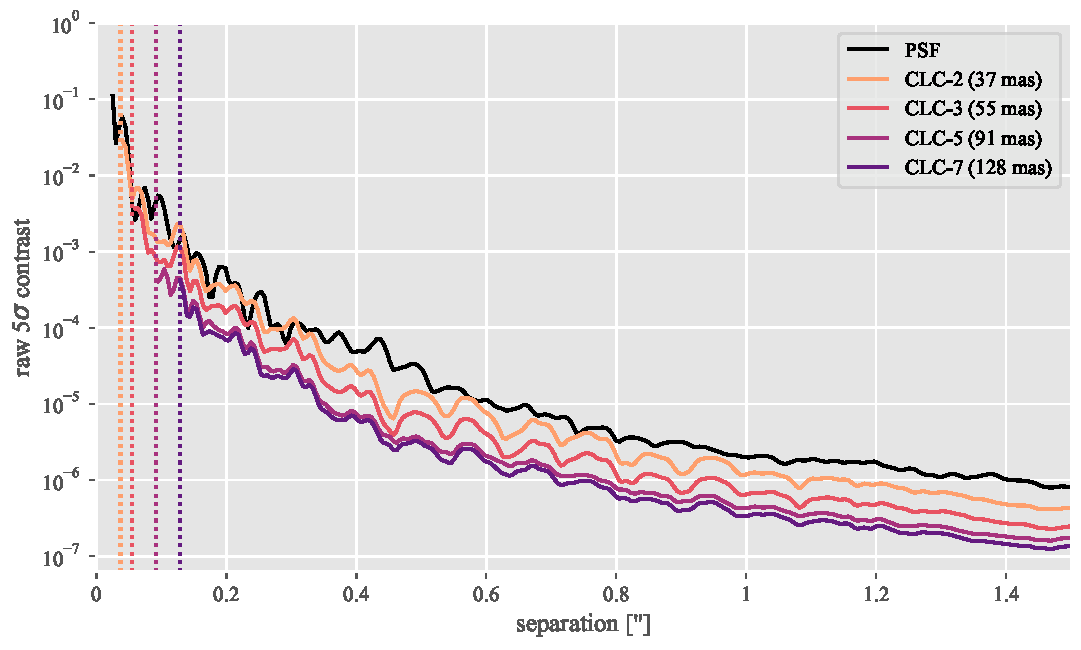
\includegraphics[width=0.95\textwidth]{figures/simulated_curves}
   \caption{Raw 5$\sigma$ contrast curves for an unocculted PSF (black line) and for each focal plane mask size (orange to purple lines). These curves are calculated from images simulated with \texttt{HCIPy}. The mask inner working angles are marked by vertical dotted lines}\label{fig:sim-contrast}
\end{figure*}

\subsection{Construction and Installation}\label{sec:install}

We chose a metallic vapor deposition process (\url{https://opto-line.com/}) for both the focal plane masks and the Lyot stop. The patterns are deposited onto a glass substrate with micrometer-precision, giving us great flexibility and precision in our designs. One downside of this approach is that the glass focal plane mask will shift the focus since it is in a converging beam. In VAMPIRES, there is a custom optics mount in the focal plane with 8 mm x 8 mm slots, so we arranged for four masks to be diced from a single 30 mm anti-reflection (AR) coated optical flat (\href{https://www.edmundoptics.com/p/30mm-dia-4mm-thick-nir-i-coated-lambda10-fused-silica-window/27562/}{Edmund Optics \#84-466}), making sure each segment was within the clear aperture. The focal plane mask patterns were deposited with chromium with thicknesses of 110 nm. The thickness was determined from the optical penetration depth for a desired transmission
\begin{equation}
    \hat{s}(\lambda) = -\frac{\lambda}{4\pi\tilde{k}(\lambda)}\ln{\frac{I(\lambda)}{I_0(\lambda)}}
    \label{eqn:throughput}
\end{equation}
where $\hat{s}$ is the thickness, $\lambda$ is the wavelength (tested across the 600-800 nm range for VAMPIRES), $\tilde{k}$ is the extinction coefficient, and $I/I_0$ is the relative intensity for transmitted light. For each of the four mask radii, we constructed a mask with 1e-8 transmission and 0.1\% transmission, which corresponds to thicknesses of 300 nm and 110 nm of chromium, respectively.

The Lyot stop was deposited onto a 25 mm AR-coated optical flat (\href{https://www.edmundoptics.com/p/25mm-dia-3mm-thick-nir-i-coated-lambda10-fused-silica-window/27561/}{Edmund Optics \#84-465}) with no further processing. We designed the Lyot stop to be reflective for the purposes of alignment and low-order wavefront sensing from the rejected light. We chose gold on its first surface for its high reflectivity ($>$90\%) across the 600-800 nm wavelength range. Following advice from our vendor, this gold layer was deposited on top of a layer of chromium which adheres better to AR coatings than gold. We used \autoref{eqn:throughput} with a linear combination of 50\% chromium and 50\% gold to determine a combined thickness of 285 nm for 1e-8 transmission. The final thickness of the chromium and gold deposit was specified as 300 nm.

The focal plane masks and Lyot stop were installed on SCExAO in January, 2022. We decided to only install the four  transmissive (0.1\%) focal plane masks given the limited number of slots in the focal plane mount. The Lyot stop was accidentally mirrored with respect to the pupil and was not correctly scaled to the beam width. A new stop was designed and procured to address these issues and was deployed on SCExAO in February, 2022.

\begin{figure*}
   \centering
   \subfloat{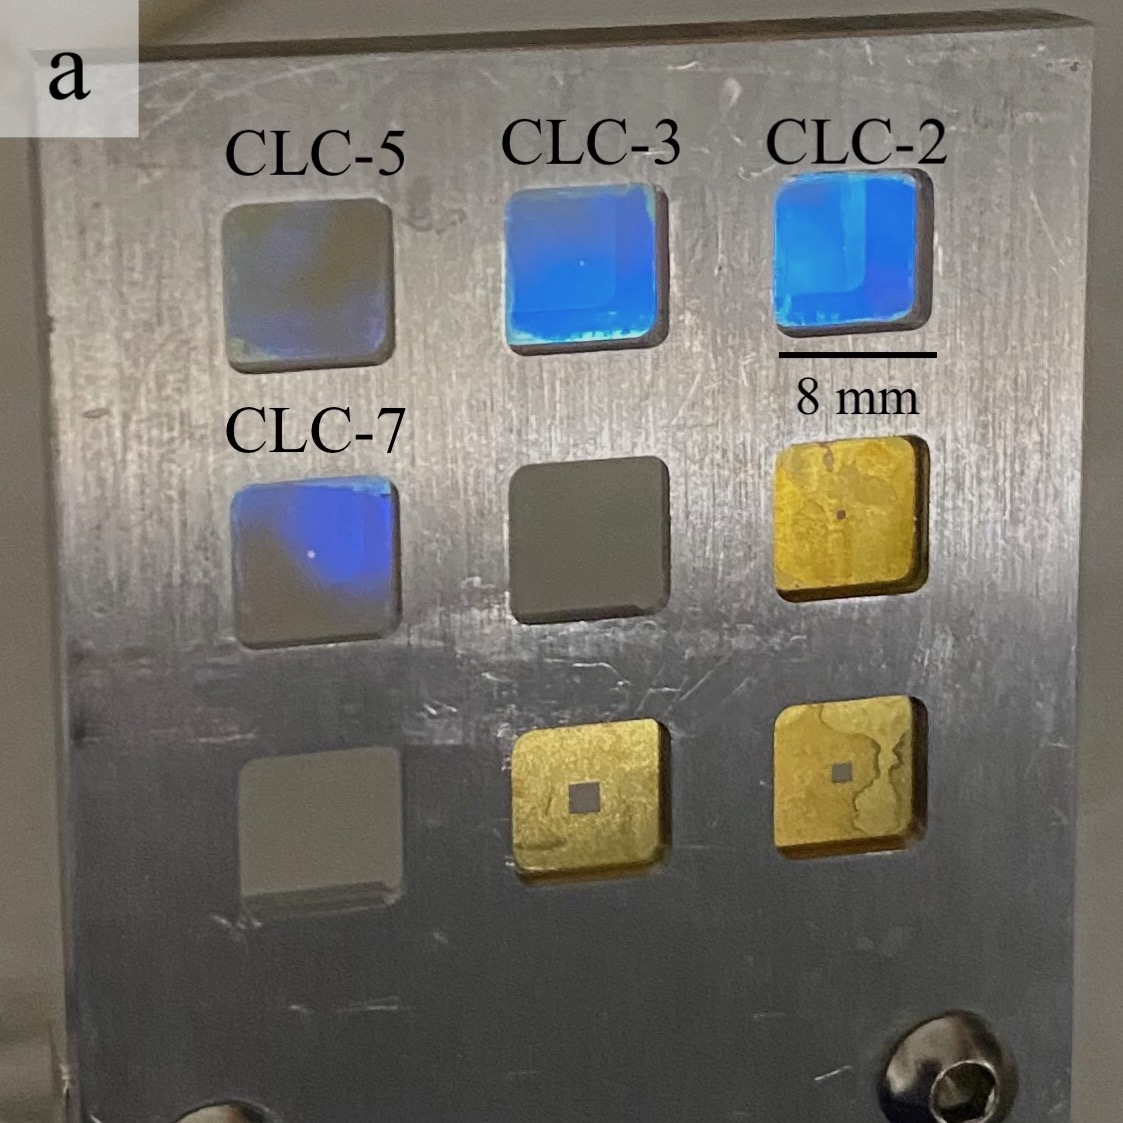
\includegraphics[width=2.5in]{figures/fpm.jpeg}}\hspace{0.5in}
   \subfloat{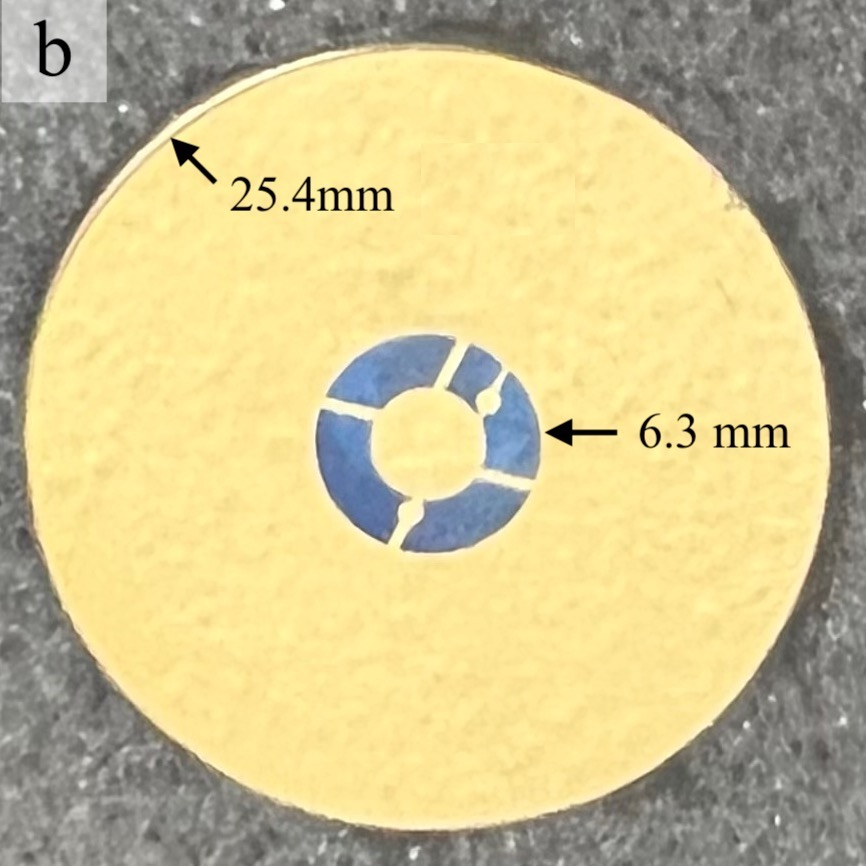
\includegraphics[width=2.5in]{figures/lyot_stop.jpeg}}
   \caption{(a) The four focal plane masks mounted in the custom-machined focal plane mount for VAMPIRES. The size of each square is 8 mm x 8 mm. (b) The undersized Lyot stop with its reflective gold coating. The dimater of the glass substrate and stop outer diameter are marked.}\label{fig:optics}
\end{figure*}

\section{Operation and Characterization}\label{sec:tests}

Both the focal plane masks and Lyot stop are installed in mounts with precise motor controllers for alignment. We found that the Lyot stop, being in the collimated beam, stays consistently aligned in-between instrument cranings (see Lozi Subaru beamsplitter paper). The focal plane masks take around a minute to manually align using a text user interface (TUI) on a high signal to noise ratio target. In addition, because the focal plane masks introduces refractive material in a converging beam, the focal point of the instrument shifts and an automatic focus measurement is performed with an offset focal plane mask before use.

\subsection{Artifical Calibration Speckles (``Astrogrid'')}

A common problem with coronagraphic imaging is accurately determing the flux and position of the host star while behind the focal plane mask. By adding sinusoidal patterns to the deformable mirror (DM) copies of the stellar PSF will appear off-axis depending on the frequency of the sinusoidal pattern\cite{sahoo2020}. These patterns are modulated in two ways: first the patterns are modulated spatially by half a wavelength to average effects of atmospheric seeing on the speckles during a typical integration. Second, the pattern is spatially modulated to create alternating sets of two PSFs, for a total of four calibration speckles equidistant from the star. The brightness of these ``satellite spots'' is proportional to the amplitude of the DM perturbation, which can be calibrated to give accurate relative photometry between the spots and the star. SCExAO/CHARIS has sucessfully demonstrated this method with astrometric precision $\sim$1.7 mas and photometric precision $\sim$0.3\%\cite{currie2020}. Examples of the ``astrogrid'' on VAMPIRES are shown in \autoref{fig:satellite-spots}.

\begin{figure*}
   \centering
   \subfloat{\includegraphics[width=3in, height=3in]{example-image-empty}}\hspace{0.1in}
   \subfloat{\includegraphics[width=3in, height=3in]{example-image-empty}}
   \caption{``Astrogrid'' calibration speckles (a) on bench (b) on sky}\label{fig:satellite-spots}
\end{figure*}

\subsection{Coronagraphic throughput}

The throughput of the coronagraph is measured in two distinct parts- the throughput of the undersized Lyot stop and the off-axis throughput of the focal plane masks. The Lyot stop throughput is proportional to the unobstructed area of the mask compared to the pupil. From the CAD drawings, the ratio of areas is 63.7\%. We measured the throughput using the pupil-imaging camera with the calibration light source, comparing the total intensity measured with a mirror (100\% of the incident light) and the Lyot stop (blocked light only). From this measurement, the Lyot stop has a throughput of 65.7\%.

The off-axis coronagraphic throughput was measured by gradually moving the mask off-axis from the calibration source. The fluxes from all of the images were normalized so the maximum off-axis flux was 1 and the on-axis flux was 0 (\autoref{fig:throughput}). Then, these curves were fit to a logistic function, allowing precise determination of the inner working angle (IWA), where the throughput is 50\%. The IWAs for each mask are 37, 55, 91, and 128 mas, respectively, which are in good agreement with the radii of the masks.


\begin{figure*}
   \centering
   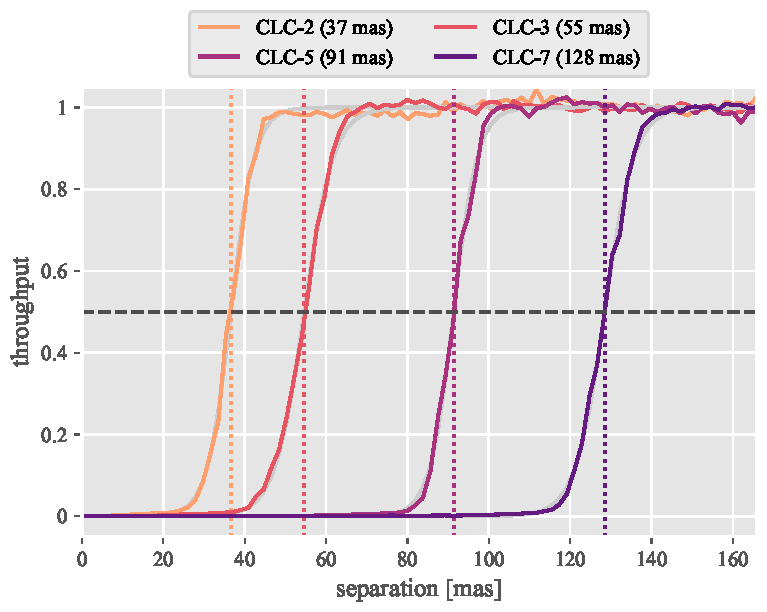
\includegraphics[height=4in]{figures/throughput_curves}
   \caption{Off-axis coronagraphic throughput for each focal plane mask. The flux throughput is normalized between 0 and 1. 50\% throughput is marked with a black dashed line, and the inner working angles, fit using a logistic function (light gray lines), are denoted by the orange to purple dotted lines.}\label{fig:throughput}
\end{figure*}

\section{Results}\label{sec:results}

\subsection{Testbed results}\label{sec:testbed}

Our first tests use the calibration source on SCExAO for determining the contrast of the coronagraph for each focal plane mask. For these tests we used the 750-50 filter since it has the highest throughput. In addition, for all tests we applied an astrogrid with 50 nm amplitude with a spatial frequency of XX\todo{find out this number}, which roughly corresponds to $\sim$15.9$\lambda/D$. We used an EM gain of 300 with optical neutral-density filters when appropriate to avoid saturating the EM-CCDs.

First, we took non-coronagraphic data allowing us to characterize both the photometry and astrometry of the astrogrid speckles as well as giving a non-coroangraphic PSF for measuring the relative attenuation from the focal plane masks. For data reduction, we used a series of 1000 images median-combined before analysis. For the astrogrid calibration, we used a hierarchical model of five two-dimensional Moffat functions
\begin{equation}
   \label{eqn:moffat}
   f(x, y | x_0, y_0, \Gamma, \alpha, I_0) = I_0 \left[1 + \frac{\sqrt{\left(x-x_0\right)^2 + \left(y-y_0\right)^2}}{\Gamma} \right]^{-\alpha}
\end{equation}
where $(x_0, y_0)$ is the center of the PSF, $I_0$ is the peak amplitude, $\Gamma$ is the half-width at half-maximum (HWHM), and $\alpha$ is the exponential scaling factor, typically close to unity. In our hierarchical model each PSF shares the $\Gamma$ and $\alpha$ parameters, and each of the four satellite spots share an amplitude. From this model, we determined the relative photometry of the 50 nm amplitude astrogrid to be XX and the radial offset to be XX $\lambda/D$.\todo{astrogrid results}

Then, we inserted the Lyot stop and focal plane masks, refocused by offsetting the mask, then centered the mask by hand. Again, we took series of 1000 images and median-combined them before processing the contrast. To measure the photometry, which has changed from the non-coronagraphic PSF due to the insertion of the Lyot stop, we fit a hierarchical model of four two-dimension Moffat functions (\autoref{eqn:moffat}). This follows the same procedure as above with shared shape parameters and intensity, but this time the stellar PSF itself is not fit. Then, we measure the photometry of each satellite spot using circular apertures with radii of $5\cdot\Gamma$ ($2.5\cdot$FWHM) and scaled using the relative intensity fit in our non-coronagraphic data.


\begin{figure*}
   \centering
   \includegraphics[width=0.8\textwidth,height=2.6in]{example-image-empty}
   \caption{Contrast and throughput curves for each mask size}\label{fig:contrast}
\end{figure*}

\subsection{On-sky results}\label{sec:onsky}


\begin{figure*}
   \centering
   \subfloat{\includegraphics[width=0.8\textwidth,height=2.6in]{example-image-empty}}
   \caption{Contrast curve for 3$\lambda$/D mask in average seeing of HDXXXXXX}\label{fig:onsky-contrast}
\end{figure*}

\section{Conclusions}\label{sec:conclusions}

In this paper we have described the design, construction, and deployment of a visible-light Lyot coronagraph on SCExAO/VAMPIRES.

In the future, as wavefront control improves for SCExAO, we want to explore phase-based focal plane masks such as the four-quadrant phase mask (4QPM)\cite{rouanFourQuadrantPhase2007}. Phase-based masks offer improved contrast over amplitude-based designs like the classic Lyot style, but are highly sensitive to pointing errors and thus require fine tip-tilt control for effective use\cite{huby2017}. We are also interested in exploring apodized Lyot stops to achieve similar or improved performance in the presence of aberrations without sacrificing as much throughput.

%%%%% Appendix %%%%%

\appendix    %>>>> this command starts appendixes


\section{Code and Data Availability}\label{sec:code}

The code used for simulating the coronagraph (\autoref{sec:design}), reducing and analyzing testbed (\autoref{sec:testbed}) and on-sky data (\autoref{sec:onsky}), and for producing the figures in this paper are all available under an open-source license in a GitHub repository (\href{https://github.com/mileslucas/vampires-coronagraph}{mileslucas/vampires-coronagraph}). The CAD drawings for the focal plane masks and Lyot stops are also available in the online repository. Further requests or questions about code or data are welcomed.

\acknowledgments

We wish to recognize and acknowledge the significant cultural role and reverence that the summit of Maunakea has always had within the indigenous Hawaiian community. We are most fortunate and thank the community for the privilege to conduct observations from this mountain. We also would like to thank Paul Sumner for his useful advice during the construction of the Lyot stop and focal plane masks. Lastly, we thank Jonathan Williams, Thayne Currie, and Timothy Brandt for generously offering observation time to use VAMPIRES for additional characterization of the coronagraph on-sky. This work is based on data collected at Subaru Telescope, which is operated by the National Astronomical Observatory of Japan. The development of SCExAO was supported by the Japan Society for the Promotion of Science (Grant-in-Aid for Research \#23340051, \#26220704, \#23103002, \#19H00703, and \#19H00695), the Astrobiology Center of the National Institutes of Natural Sciences, Japan, the Mt Cuba Foundation and the director's contingency fund at Subaru Telescope. This research was funded by the Heising-Simons Foundation through grant \#2020-1823.

%%%%% References %%%%%

\bibliography{report} % bibliography data in report.bib
\bibliographystyle{spiebib} % makes bibtex use spiebib.bst

\end{document}
